%  
%  in CH1 give an real life example at the begining as a BACKGROOUND
%  describe bacis concepts
%  and go into more details? obvious
%  
%  
%  
%  in CH2 active learning or web optimization
%  
%  
%  
\documentclass[12pt, a4paper, pdflatex]{report}
%  notitlepage - abstract on the same page
\usepackage{indentfirst} % indent frst paragraph of section
\usepackage{fullpage}    % full A4 page
\usepackage{amsmath}
\usepackage{amsfonts}    % fancy maths font
\usepackage{mathrsfs}    % fancy maths font
\usepackage{dsfont}      % indocator finction

\usepackage[pdftex]{graphicx}
\usepackage{cite} % BiTeX
\usepackage{lipsum}
\newcommand{\ts}{\textsuperscript}
\usepackage[usenames,dvipsnames]{color}

% for multi figures
\usepackage{graphicx}
\usepackage{caption}
\usepackage{subcaption}

\usepackage[]{algorithm2e}

% \usepackage{polski}
% \usepackage[polish,english]{babel}
% \usepackage[utf8]{inputenc}
\usepackage[T1]{fontenc} % polsih

% Code snippets
\usepackage{listings}
% \usepackage{color}


\definecolor{dkgreen}{rgb}{0,0.6,0}
\definecolor{gray}{rgb}{0.5,0.5,0.5}
\definecolor{mauve}{rgb}{0.58,0,0.82}

\lstset{frame=tb,
  language=R,
  aboveskip=3mm,
  belowskip=3mm,
  showstringspaces=false,
  columns=flexible,
  basicstyle={\small\ttfamily},
  numbers=none,
  numberstyle=\tiny\color{gray},
  keywordstyle=\color{blue},
  commentstyle=\color{dkgreen},
  stringstyle=\color{mauve},
  breaklines=true,
  breakatwhitespace=true
  tabsize=3
}
% END Code snippets

% $\backsim\ \sim\ \thicksim$

\newcommand{\HRule}{\rule{\linewidth}{0.5mm}}

\newenvironment{dedication}
  {\clearpage           % we want a new page
   \thispagestyle{empty}% no header and footer
   \vspace*{\stretch{1}}% some space at the top 
   \itshape             % the text is in italics
   % \raggedleft          % flush to the right margin
   \raggedright          % flush to the right margin
   \par\setlength{\leftskip}{0.3\textwidth}\noindent\ignorespaces
  }
  {\par % end the paragraph
   \vspace{\stretch{3}} % space at bottom is three times that at the top
   \clearpage           % finish off the page
  }

\begin{document}

\begin{titlepage}
\begin{center}
% Upper part of the page. The '~' is needed because \\
% only works if a paragraph has started.

\includegraphics[width=0.5\textwidth]{graphics/UOB-logo.png}~\\[4cm] % was 1cm

% \textsc{\LARGE University of Bristol}\\[1.5cm]

%\textsc{\Large Final year project}\\[0.5cm]

% \colorbox{magenta}{problem}

% Title
\HRule \\[0.4cm]
{ \huge \bfseries \emph{Multi-armed bandits.}\\
	Comprehensive introduction to the topic with \emph{Thompson's Sampling} approach\\
  \&\\
  Active Learning in the bandits scenario.\\[0.4cm] }
\HRule \\[1.5cm]

% Author and supervisor
\begin{minipage}{0.4\textwidth}
\begin{flushleft} \large
\emph{Author:}\\
Kacper B. \textsc{\textbf{Sokol}}
\end{flushleft}
\end{minipage}
\begin{minipage}{0.4\textwidth}
\begin{flushright} \large
\emph{Supervisor:} \\
Dr.~David \textsc{\textbf{Leslie}}
\end{flushright}
\end{minipage}

\vfill

% Bottom of the page
{\large \today}
\end{center}
\end{titlepage}

% \title{\emph{Multi-armed bandits} problem.\\
% 	Practical introduction to the problem for everyone.\\
% 	Real life application.}
% \author{Kacper Sokol\\University of Bristol, UK}
% \date{\today}
% \maketitle
% \begin{flushright}
% Supervised by:\\
% \textbf{David Leslie}
% \end{flushright}
% \begin{center}
% \line(1,0){250}
% \end{center}

\begin{abstract}
\thispagestyle{empty}% no header and footer
This dissertation consists of two chapters. First one is a comprehensive introduction to theory underlying multi-armed bandits problem. Reader is assumed not to need any prior knowledge in this field, only basics of statistics and probability theory are required. Second chapter is experimental part focused on ...
\begin{center}
Keywords: \textbf{multi-armed, bandit, active, semi-supervised, learning, exploration, exploitation, Thompson's sampling}
\end{center}
\end{abstract}

\begin{dedication}
I would like to thank my parents who support me both financially and mentally. For the guidance and advice they are providing so I can make right choices throughout life and fulfill my dream of studying abroad.\newline

It would also be a painful journey without my supervisor Dr.~David~Leslie who always served me with an advice how to ``read'' all the mathematical books not to get overwhelmed with heavy maths.\newline

Finally, big thanks to I.\ and J.\ who always take care of my leisure time even though it always lacks.\\[2cm]


% \foreignlanguage{polish}{}
\begin{flushright}
Dzi\k{e}kuj\k{e} mamo,\\
dzi\k{e}kuj\k{e} Tomek.
\end{flushright}



% I was lost now I'm found
\textcolor{white}{found me!}



\end{dedication}


\newpage
\tableofcontents
% \newpage
\thispagestyle{empty}
\cleardoublepage
\pagestyle{plain}
\setcounter{page}{1}


\chapter{\texttt{\textbf{Exploration}} of multi-armed bandits theory.}
The \emph{multi-armed bandit} problem has been rapidly developing field of statistics and probability theory since early 20\ts{th} century. With a vastly growing number of \colorbox{magenta}{problems} that could be framed as a multi-armed bandit scenarios the field has become interest of many scientists, researchers, economists not to mention companies looking for work efficiency improvement and savings. All the solutions addressing these \colorbox{magenta}{problems} can be expressed as simple as finding a balance between \emph{exploration} and \emph{exploitation}.


\section{Background}
Many people know statistics and probability as analyzing processes or data in various aspects. They consider it as a rather \emph{static} science. But what if the process of our interest is continuously developing while we want to discover it or it demands our interaction. Simple statistics or probability might not be able to handle such cases as good as bandit theory.\\

To begin with, lets consider \emph{fruit machine} as it is a first thing that crosses reader's mind after hearing about multi-armed bandits. Imagine a row of slot machines in front of you. Pulling an arm of each of these automaton will result in different outcome (win or loose) each with corresponding probability according to some unknown distribution. Result for now on can be interpreted as various reels combinations. For the sake of simplicity it can be assumed that each automaton gives binary result: \emph{win} with probability $p$ and \emph{loose} with probability $p-1$. Without lost of any information row of such machines can be transformed into only one automation but with multiples arms or buttons each corresponding to single machine in a mentioned row.\\

The natural example that follows binary bandits is a row of coins, where some of them may be unfair. In presented scenario each coin corresponds to an \emph{Arm} of a bandit and tossing one of them for several times can be considered as realization of a Bernoulli process with unknown parameters.\\ If a player is rewarded when the outcome of a trial is \textbf{H}ead then the goal is to find the coin which has bias with maximum probability of \textbf{H} and play it forever.\\

If a gambler does not want to loose all possessed money really quick it would be probably a good idea to have some kind of strategy that maximizes chances of winning. It is assumed that the gambler is for the first time in a given casino so any prior information regarding expected return from each of the arm is assumed to be unknown. Initially random arm is chosen as all of them "look the same". On contrary, during the second turn selecting \emph{optimal} arm to play on becomes a serious dilemma that you might have not yet realized. The gambler faces a choice between already pulled arm with sample of expected return that is known and any other arm which for now on seem "the same" as there is no information about potential reward.\\
If gambler decides to take advantage of already known arm and pull it again we call this action \emph{exploitation}--- taking advantage of already checked possibilities. On the other hand, taking a risk and choosing one of unknown arms will result in gathering some more information about the system what is usually said to be \emph{exploration} step.\\

ADD-ON
Multi-armed bandit are class of problems originated from a sequential allocation dilemmas. They were formulated during Second World War and quickly became recognized as so difficult to solve that they were put aside. First general solution was formalized by John Gttins\ref{sec:gitind} in late 60's nevertheless, it was not widely known until the early 80's.~\cite{gittins+glazebrook+weber}


\section{Applications} % emphasized underlying
Multi-armed bandits is not just theory that one reads from a book and try to memorize, but it extends to many real life applications. This section is devoted to simple case study in which it seems natural to use "bandit approach". Applications are versatile ranging from drug testing and maximizing income from web advertisement through semi-supervised machine learning in modern computer science as well as time and budget management of research projects.\\

To begin with, imagine a clinic testing two new drugs for a certain disease. Patients are queuing up to receive a treatment. Assuming that doctor cannot refuse to treat anyone, for each person suffering from a disease (each \emph{Play}) there are two possible cures (two \emph{Arms}). The key assumption here is that the effect of chosen action occur immediately, in other words treated person either stays sick or the disease goes away (immediate \emph{Payoff}). The goal of a doctor is to maximize the number of cured people. This model defines two-armed bandit.\\

The second mentioned approach is nowadays widely incorporated by companies such as Google~\cite{AYPSze12}\cite{ASMB:ASMB874}, LinkedIn~\cite{Tang:2013:AAF:2505515.2514700}, Microsoft~\cite{graepel2010web}, Yahoo~\cite{Li:2010:CAP:1772690.1772758} to their services. Research groups of these companies are using bandits algorithms to choose best website layout and advertisements locations to increase "click-rate", improve recommendation systems or enhance performance of semi-supervised and active learning algorithms in a field of machine learning.\\

The bandit theory also plays a key role in experiment allocation with restricted time and budget~\cite{gittins+glazebrook+weber}. While considering research projects pending to be conducted with limited amount of resources such as scientist time and grant funding as \emph{Arms} of a bandit. The goal is to maximize the number of accomplished projects (\emph{Payoff}) before running out of money.\\

With all the above scenarios barely scratching the tip of the iceberg we are now focusing on foundations of multi-armed bandits theory that one needs to precisely describe the processes happening "behind the scene".

\section{Structure of this chapter}
We begin with introducing the reader with necessary notation and nomenclature. Then we are moving to basic process description. Next proved optimal solutions of multi-armed bandits problem are described. Finally we form conclusions and highlight ongoing research with possible results and influence on applications.


\section{Terminology}
More scientific definition of "simple" multi-armed bandit in a statistical decision theory defines it as: sequential selection from $N \geq 2$ stochastic processes--- generally called \emph{Arms}, where both time and processes may be discrete or continuous. The goal is typically to recover unknown parameters which characterize stochastic processes behind each of the \emph{Arm} to maximize expected \emph{Payoff}.

It is very useful to be familiar with most common terms used to describe multi-armed bandit in papers and books. The basic concepts are listed below.
\begin{description}
\item[Multi-armed bandit ($N$)]--- a ``device'' with $N \geq 2$ possible choices of action (\emph{Arms}).
\item[Strategy ($\tau$)]--- tells the \emph{Agent} which \emph{Arm} to pull at given stage of \emph{Game}. A strategy is \emph{optimal} if it yields maximal expected \emph{Payoff}.
\item[Arm]--- one of $N$ actions that may be taken by \emph{Agent}. An \emph{Arm} is \emph{optimal} if it the best selection when following some \emph{optimal} strategy.
\item[Play]--- an \emph{Arm} pulled at stage $m$ of the \emph{Game} (i.e.\ one turn).
\item[Agent]--- a person that decides which \emph{Arm} to pull based on \emph{Strategy} $\tau$.
\item[Game]--- a sequence of \emph{Arms} pulled based on chosen \emph{Strategy} $\tau$.
\item[Payoff]--- a return of a game such as \emph{win--loose} or \emph{amount} of money gained.
\item[Discount series]--- factors that define how valuable is each of \emph{Payoffs}. For example only first $m$ outcomes may count and all the rest is neglected or the longer the \emph{Game} is ran the less particular outcome counts toward overall expected \emph{Payoff}.
\end{description}


\section{General assumptions}
Two fundamental assumptions to vast majority of bandit problems regard benefits from selecting an arm, namely:
\begin{itemize}
\item immediate \emph{Payoff} i.e.\ \emph{Agent} knows result of taken action straight away,
\item information gathered after a \emph{Play} can be used to modify chosen \emph{Strategy}.
\end{itemize}
Moreover in some cases we may restrict the memory of an \emph{Agent} to last $s$ outcomes. Therefore, selected \emph{Strategy} $\tau$ can relay on up to $s$ previous \emph{Plays}. These bandits approaches are called \emph{finite memory}.\\
Majority of this dissertation assumes that \emph{Arms} are independent. If this setting changes it will be clearly stated.


\section{Discount Sequence}
To specify the rules governing the ``significance'' of outcome from a single play at stage $m$ the \emph{discount sequence} is introduced. It is a vector $\mathbf{A}$ of specified length, which can also be infinite.
$$
\mathbf{A} = \left( \alpha_1, \alpha_2, \alpha_3, ... \right)
$$
When an \emph{Arm} is selected the discount sequence is modified as follows:
$$
\left( \alpha_1, \alpha_2, \alpha_3, ... \right)
\rightarrow
\left( \alpha_2, \alpha_3, \alpha_4, ... \right)
$$

\subsection{Observable and non-observable sequences}
\lipsum[1]


\subsection{Most common sequences}
There are many different discount sequences used with multi-armed bandits each with numerous assumptions. In the literature only two of them are described in great detail and both are presented below.
{
\subsubsection{Uniform sequence}
This discount sequence is most commonly used when a player wants to maximize the payoff of first $h$ outcomes.
The $h$-horizon uniform discount sequence is defined as:
\[
 \alpha_i =
  \begin{cases}
   1 & \text{for } i \leq n \\
   0 & \text{for } i > n
  \end{cases}
\]
leading to:
\[
  \mathbf{A} = ( \underbrace{ 1, 1, 1, ..., 1}_{h\text{ elements}}, 0, 0, 0, ... ) \text{ .}
\]\\
\\
Here after \emph{Arm} selection the horizon of discount sequence is decreased by $1$.


\subsubsection{Geometric sequence}
The geometric discount sequence is expressed with components $\alpha_i = a^{i-1}$ for some $a \in ( 0, 1 )$ resulting in:
$$
\mathbf{A} = \left( a^0, a^1, a^2, ... \right)
$$
where $\alpha_1 = a^0$ is always equal to $1$.\\
\\
On the other hand, here after \emph{Arm} selection the discount sequence is proportional to original sequence.\\
\\

}
In case of both sequences the decision problem and optimal strategy is unchanged if a discount series is multiplied by some constant. Furthermore, in case of geometric sequence is effectively the same the same throughout the \emph{Game}.

\subsection{Random discounting}
\subsection{Infinite horizon }

\subsection{Non-monotone sequences}



\section{Bandits settings}
\subsection{Real time, random bandits}
\subsection{Information gathering}
\subsection{Dependant \emph{Arms}}



\section{Seeking optimal solution}
In this section I will present number of approaches to find and optimal solution.\\
Blah blah blah blah.
Strategy id balancing exploration and exploitation to find optimal solution. Sometime it demand sanctifying early payoff to gain some more information about the system and maximize future payoff.
Information vs.\ immediate payoff. -- in hospital example case it means that sacrificing good of early coming patients by means of experimenting means improvement over time and better results of treatment on future patients.
To democratize it we can use geometric sequence so health of current patients is the same in comparison to future patients.\\
\\
\\
OPTIMALITY IS GUARANTEED BY LIMIT ... ETC.
\\
\\
This result shows that when the discounting is geometric, a bandit problem involving k independent arms can be solved by solving k different two-armed bandits, each involving one known and one unknown arm.\\

\subsection{Index approach (Gittins Index)\label{sec:gitind}}
% chap 1
It is one of the oldest approaches providing solution to long before formulated and pioneering work of indeed Gittins of the index moved forward not only mult-armed bandits concept but whole wide class of sequential allocation problems.\\

The basic intuition behind this approach is to assign \emph{priority indices} to each action, where index of particular action should only depend on the history of outcomes for this action and no other. The decision process then comes down to choosing action with highest current index.\\

Basic theory of allocating indeces is based on calibrating actions at given state against some standardized actions with simple properties. The main advantage of such approach is restricting state function of an action to depend only on one's own history therefore deducing the complexity.\\

So there exists a real valued function defined by a set of all available alternatives, and the selected one is chosen to maximize this function. This function is(are) dynamic allocation index(ices). indeces are described as functions on the set of available alternatives.\\
With such indeces we can specify optimal policy for particular problem which has any set of possible alternatives of a given type.\\

Defining optimal policy- the one that chooses optimal arm infinitely many times- is obscure(not straight forward) in \emph{preemptive} case --- what means that arbitrary switching between actions is allowed which take negligible time, 

all is with regard to so called \emph{standard bandit problem}

% beg chap 2
in the simplest case we consider multi-armed bandit as a number of semi-Markov decision processes. The \emph{index theorem} states that there exists \emph{index policy} which is optimal. Wht means that there exists a real-valued index, say $\nu ( B_i , \xi_i(t) )$, where $B_i$ is i-th bandit process and $\xi_i$ is a state of i-th process. Furthermore index for particular bandit process depends only on current state of this process and no other processes. The optimal strategy is thus to continue the process with greatest index.\\

The index theorem says that a policy for bandits process is optimal if it is an index policy ith respect to $\nu(B_1, .), \nu(N_2, .), ... , \nu(B_n, .)$.\\


%intro chap 3
ASSUMPTIONS\\
The general assumptions that need to hold so we are able to apply gittin index:
* rewards are accumulated up to an infinite time horizon\\
* there is constant exponential discounting\\
* there is only one processor/server\\
******\\
* discounting is strict?\\
* unless bandit is processed (cont control is recived) no rewards accrue from it and its state does not change\\

\subsection{Bayesian approach}
Bayes' theorem allows for "straight forward" application to adaptive learning so it's a good approach tool in sequential decision making 

\subsection{Strategy comparison}

\subsection{Minimax approach}

\subsection{Finite memory strategy}
\subsubsection{'Stay on a winner'}

\subsection{Myopic strategies}
Not good in general.\\

% from gittins book\\
it corresponds to maximizing the expected reward during the next infinitesimal time interval

it is called myoptic because it neglects things that may happen later or disregard a long-range(long-time) vision to continue the optic metphore.

for some class of problems it can be shown that short term optimum is simultaneously long term one so for this kindaof problems this solution works as it does not perform complex computation or doesn;t do lookahead.

% my
local not global solution with respect to time.
it can be applied to many other strategies but is most often used with index methods.

\subsection{Thompson Sampling approach}
As all the rest of methods is well described in literature and they were main subject of interest it is relatively easy to find good texts about them. On contrary, Thompson Sampling is cutting edge approach with a lot of research going on the focus will be put on it and it will be described in deep details in  \textbf{Section~\ref{sec:thompsonsampling}} which is devoted to Thompson Sampling approach to finding an optimal strategy.

\subsection{etc.\ based on Google paper}

% dynamic programming recurence equation
describing by recursiveequations--- demand significant amount of computation and memory storage<- index book.


\section{Thompson Sampling\label{sec:thompsonsampling}}
To fully develop \emph{Thompson Sampling} approach to multi-armed bandit theory, two concepts need to be introduced:
\begin{itemize}
\item Bayesian statistics \emph{and}
\item sampling theory.
\end{itemize}
It is possible to use any probability distribution with \emph{Thompson Sampling} but for the sake of simplicity we will focus in this paper only on \emph{normally} distributed data. This restriction does not mean that it is not possible to apply this technique with any other distribution but due to space constrains the theory will be presented with \emph{normal likelihood}. Furthermore, discussing other scenarios of Thompson Sampling would demand from reader to be familiar with analytic approach to Bayesian \emph{posteriors}, \emph{priors} and \emph{likelihoods}.

\subsection{Bayesian statistics}
In this section we will shortly introduce normal distribution. Then we will discuss its aspects with regard to Bayesian statistics.

\subsubsection{The normal distribution}
The most common distribution in statistics with well known bell-shaped (see \emph{Figure~\ref{fig:normaldist}}) plot is the normal distribution also called \emph{Gaussian} distribution. If a random variable $\mathrm{X}$ follow such distribution parametrized by \emph{mean} $\mu$ and \emph{standard deviation} $\sigma$ we commonly write $\mathrm{X} \sim \mathcal{N}\left( \mu, \sigma^2 \right)$. Probability density function of $\mathrm{X})$ is:
$$
f \left(x | \mu, \sigma \right) = \frac{1}{\sigma \sqrt{2 \pi }} e^{- \frac{ {\left (  x - \mu \right )}^2 }{2 \sigma^2} }
$$
where the first part ${\left( \sigma \sqrt{2 \pi } \right)}^{-1}$ is a normalizing factor and the later part is a distribution ``kernel''.
$$
\int_{-\infty}^{+\infty} \! f \left(x | \mu, \sigma \right) \, \mathrm{d}x = 1
$$
with area under curve from $-\infty$ to $+\infty$ integrating to $1$~\cite{rice1995mathematical}.


\begin{figure}[htbp]
\centering
\includegraphics[width=0.5\textwidth]{graphics/normalpdf.pdf}
\begin{tiny}
\caption{Probability density function of normal distribution $\mathcal{N}\left( 0, 5 \right)$ in characteristic bell shape created in \texttt{R} (Snippet in \emph{Appendix~\ref{snip:normaldist}}).\label{fig:normaldist}}
\end{tiny}
\vspace{1cm}
\end{figure}



\subsubsection{\emph{prior}, \emph{posterior} and \emph{likelihood} distributions}
The next concept that we introduce is the dependency between prior, posterior and likelihood of a particular distribution. To illustrate it the \emph{normal} distribution will be used for the reasons mentioned above. The generalization to other distributions is straight forward~\cite{gelman2003bayesian}.\\

The basic theorem underlying all this section is called Bayes' theorem for point probabilities and states:
$$
p \left( \mathrm{B} | \mathrm{A} \right) = \frac{  p \left( \mathrm{A} | \mathrm{B} \right) p \left( \mathrm{B} \right) }{ p \left( \mathrm{A} \right) }
$$
\begin{center}
or
\end{center}
$$
p \left( \mathrm{B} | \mathrm{A} \right) \propto p \left( \mathrm{A} | \mathrm{B} \right) p \left( \mathrm{B} \right)
$$
where:
\begin{description}
\item[$p \left( \mathrm{B} | \mathrm{A} \right)$] is \textbf{posterior}--- being conditional probability of event \textrm{B} given event \textrm{A},
\item[$p \left( \mathrm{A} | \mathrm{B} \right)$] is \textbf{sampling density (``likelihood'')}--- being conditional probability of event \textrm{A} given event \textrm{B},
\item[$p \left( \mathrm{B} \right)$] is \textbf{prior}--- being marginal probability of event \textrm{B} and
\item[$p \left( \mathrm{A} \right)$] is \textbf{marginal} probability of event \textrm{A} (data) being normalizing factor.
\end{description}

Now we will focus on general results of Bayesian statistics when our likelihood function is normally distributed. From this point onwards we can develop a couple of different scenarios described below.\\

\textbf{\textrm{Non-informative prior. }}If we are lacking information about prior distribution the best that can be done is to minimize its influence on the inference. According to \emph{principle of insufficient reason} proposed by Bayes and Laplace we should assume that prior is \emph{uniformly} distributed so all outcomes are equally likely. We also assume that it is distributed over the real line for both $\mu$ and $\log \sigma^2$ (transformation to $\log$ scale is performed because $\sigma^2$ is non-negative quantity and it results in stretch along real line). These operations result in joint probability $p \left( \mu, \sigma^2 \right) \propto \frac{1}{\sigma^2} $ leading to posterior distributions given by $p \left( \mu | \mathrm{X}, \sigma^2 \right) \sim \mathcal{N} \left( \bar{x}, \frac{\sigma^2}{n} \right) $ and $p \left( \sigma^2 | \mathrm{X}, \mu \right) \sim \mathrm{Inv}\text{-}\mathrm{Gamma} \left( \frac{n}{2} , \sum_{i} \frac{\left( x_i - \mu \right)^2}{2}  \right) $ (inverse gamma distribution). This approach is not perfect and its criticism is widely known but for our application it suffices~\cite{Syversveen98noninformativebayesian}.\\

% give equation for normal likelihood --- uniform prior

\textbf{\textrm{Informative prior. }}It is the opposite scenario to one described above. With known distribution of the prior the application of Bayesian statistics is straight forward. From this point onward we will assume that our prior is informative with normal distribution.\\

\textbf{\textrm{Known variance. }}Firstly we will consider \emph{normal prior--normal likelihood} with $\sigma^2$ known and $\mu$ unknown (our variable).
$$
f \left( \mu | \mathrm{X} \right) \propto f \left( \mathrm{X} | \mu \right) f \left( \mu \right)
$$
The $\sigma^2$ in the notation is omitted for clarity purposes. In this case out prior is defined as follows:
$$
f \left( \mu \right)    \sim   \mathcal{N}\left( \mu, \tau^2 \right)
%                        ~
$$
giving:
$$
f \left( \mu \right)    =     \frac{1}{\sqrt{2\pi} \tau} e^{- \frac{{\left( \mu - M \right)}^2}{2 \tau^2} }
$$
where $M$ is prior mean and $\tau^2$ is variance of $\mu$ round $M$; likelihood is given by:
$$
f \left( \mathrm{X} | \mu \right)     \sim    \mathcal{N}\left( \mu, \sigma^2 \right)
$$
resulting in:
$$
f \left( \mathrm{X} | \mu \right)    =     \prod_{i=1}^{n} \frac{1}{\sqrt{2\pi} \sigma} e^{- \frac{{\left( \mu - x_i \right)}^2}{2 \sigma^2} }
$$
where $x_i \in X$ are data points.\\
After plugging both of them into Bayes rule we get:
$$
f \left( \mu | \mathrm{X} \right)     \propto     \frac{1}{\sigma \tau} e^{ -\frac{ {\left( \mu - M \right)}^2 }{2 \tau^2} -\frac{ \sum_{i=1}^{n} {\left( \mu - x_i \right)}^2 }{2 \sigma^2} }
$$
what clearly contains a kernel of normal distribution. After some algebraic transformation we finally get that posterior is \textbf{normally} distributed with mean $\epsilon$ and variance $\delta^2$ ( $f \left( \mu | \mathrm{X} \right) \sim \mathcal{N} \left( \epsilon, \delta^2 \right) $ ):
\begin{eqnarray*}
\epsilon &=& \frac{\sigma^2 M + n \tau^2 \bar{x}}{n \tau^2 + \sigma^2} = \frac{ \frac{1}{\tau^2} }{ \frac{1}{\tau^2} + \frac{n}{\sigma^2} }M + \frac{ \frac{n}{\sigma^2} }{ \frac{1}{\tau^2} + \frac{n}{\sigma^2} } \bar{x} \\
\delta^2 &=& \frac{\sigma^2 \tau^2}{n \tau^2 + \sigma^2} = \frac{ \frac{\sigma^2}{n} \tau^2 }{ \tau^2 + \frac{\sigma^2}{n} } \text{ .}
\end{eqnarray*}
\\

\textbf{\textrm{Unknown variance. }}This is more realistic case with the posterior model:
$$
p \left(  \mu, \sigma^2 | \mathrm{X} \right) \propto p \left( \mathrm{X} | \mu, \sigma^2 \right)    p \left( \mu, \sigma^2 \right) \text{ .}
$$
We now need to specify the details of prior distribution. One way is to assume independent distributions of both $\mu$ and $\sigma^2$ and establish separate priors for each with $p(\mu, \sigma^2) = p(\mu) p(\sigma^2)$ what is widely documented as a good technique~\cite{gelman2003bayesian}.\\
With unknown variance one approach is to follow \emph{non-informative} prior scenario described above. The other one is to continue assumption that $\mu \sim \mathcal{N} \left( M, \tau^2 \right)$ with choice of parameters resulting in a flat distribution e.g. $M=0$, $\tau^2 = 10^4$. Furthermore, it is easy to spot that $\sigma^2$ follows \textrm{Inverse}-\textrm{Gamma} distribution with ... . Both these results leads to posterior distribution being ... .\\

Basic results that yields from Bayesian statistics for normal likelihood are available in wide variety of books. For more details regarding normal and other distributions please refer to~\cite{lynch2007introduction}\cite{gelman2003bayesian}.\\

\subsection{Sampling}
In general sampling is a technique used in statistics to select at random a subset of individuals or data points from a population of interest. To goal of such procedure is to gather representative group which holds the properties of original population. The main advantage of such approach is lowering the amount of data to process.\\
In our approach we use sampling to draw at random from particular pool (\emph{arm}) with unknown distribution.



\subsection{Introduction to Thompson Sampling}
start writing about Thompson sampling~\cite{May:2012:OBS:2503308.2343711}.




\begin{figure}[htbp]
\centering
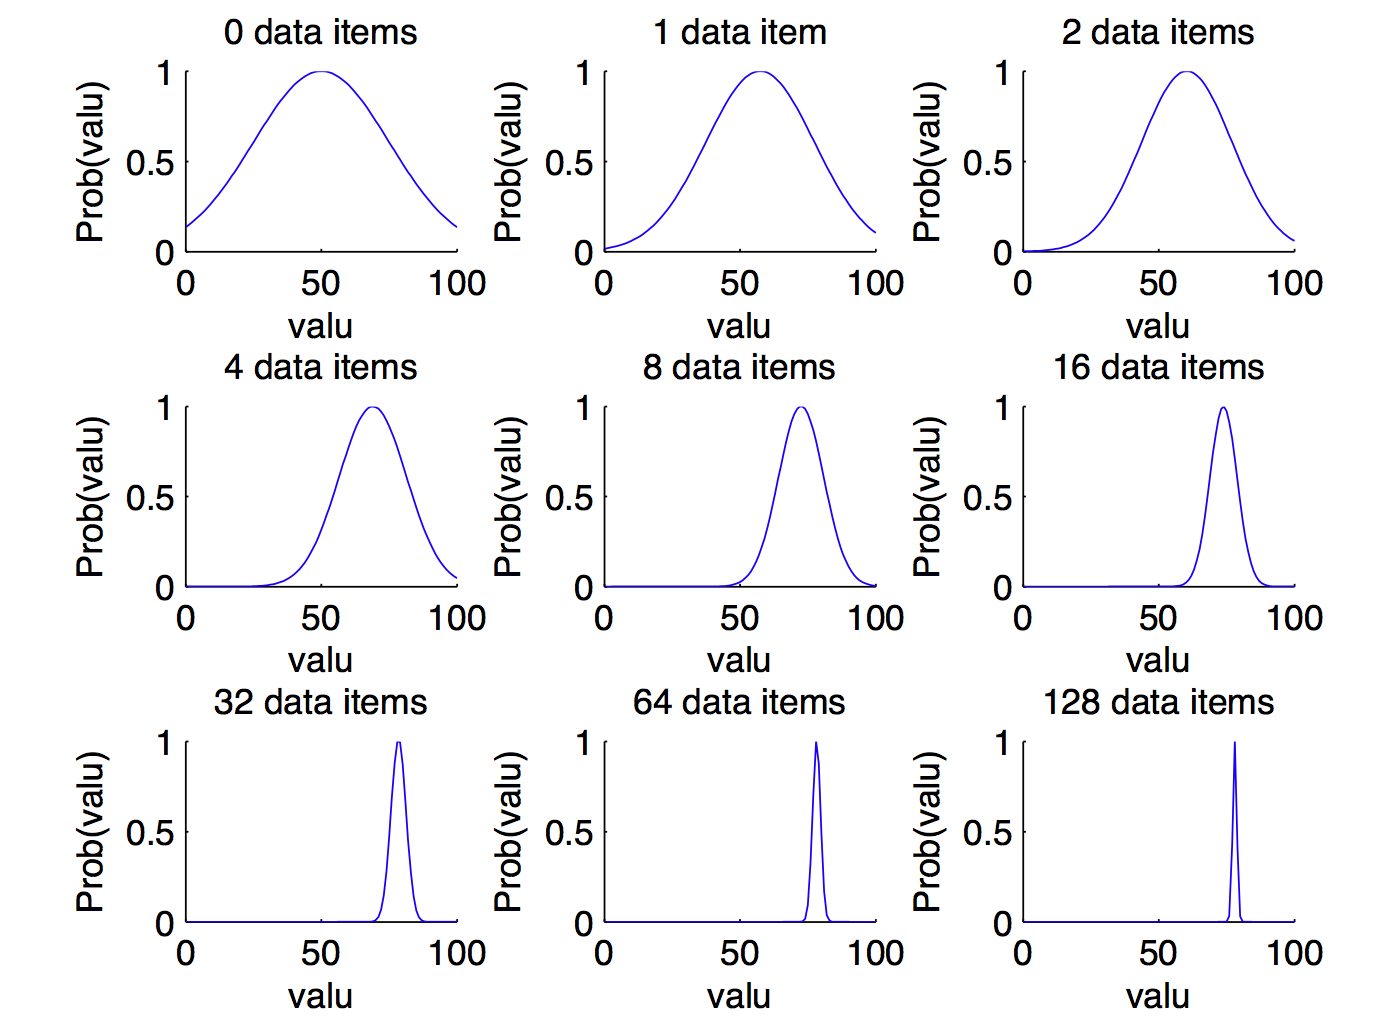
\includegraphics[width=0.7\textwidth]{graphics/sampling.png}
\begin{tiny}
\caption{Sampling and updating posterior probability density function of normal distribution $\mathcal{N}\left( \mu , \sigma^2 \right)$ (Figure taken from~\cite{Jacobs2008normalnormal}).\label{fig:sampling}}
\end{tiny}
\vspace{1cm}
\end{figure}








\chapter{\texttt{\textbf{Exploitation}} --- Practical application}

There is a number of historical applications of multi-armed bandits(MAB) concerned mainly with research time management, general job-scheduling, economics and military~\cite{gittins+glazebrook+weber}.
Nowadays one of main utilisations is found in contextual bandits which are foundations for optimizing online advertising income. The general idea behind this concept is to present different variations of ads layout at given webpage which are suited to user by inspecting one's history and are widely used by IT giants like Google, Yahoo, Facebook, LinkedIn or Microsoft. For majority of these companies this theory is of high interest as lion's share of their revenue flows from click-through rate in online advertising.~\cite{graepel2010web, Scott:2010:MBL:1944422.1944432}\\

Other, most recent application of MAB theory fitted into computer science world is concerned with classification issue in environment of insufficient information. This approach to machine learning field seems to be under-explored and needs more attention from a research world as to the best of our knowledge it was addressed so far in only one scientific publication, namely~\cite{DBLP:journals/corr/GantiG13}.\\
Our decision was to pursue this topic mainly by presenting here deep analysis of chosen in~\cite{DBLP:journals/corr/GantiG13} approach. After broad explanation we seek for potential improvements and alternatives of presented algorithm.

\section{Structure of this chapter}
We first introduce foundations of machine learning needed to develop concepts of semi-supervised(SSL) and active(AL) learning. Next, we introduce whole family of active learning scenarios and give detailed description of the chosen one. Then, we present possible connection between processes of MAB and AL. This interface, will allow to frame active learning scenario as bandit process.\\
Proceeding, main section of this chapter focuses on described in \cite{DBLP:journals/corr/GantiG13} ``bridge'' connecting both worlds. Finally, we explore potential changes that can be introduced and improvements that can be beneficial for described earlier algorithm.
%explore in great detail

\section{Machine Learning 101}
\subsection{General Learning}
Machine Learning is a field of Computer Science which is mainly concerned with building a model for a given data. Classification problem is of the form $\mathit{l} : \mathscr{X} \rightarrow \mathscr{Y}$, where $\mathscr{X}$ is called \emph{instance space} and $\mathscr{Y}$ is \emph{output space} --- in supervised scenario often replaced with $\mathscr{L}$ and called \emph{label space}.\\
Such function $\mathit{l}$ is called \emph{model}, which we try to approximate. The instances which are supplied to the model are preprocessed to extract \emph{features}, which represent each instance in a form of a vector describing chosen attributes. Based on feature vector given model assigns the element to particular region in output space; or in case where $\mathscr{Y} = \mathscr{L}$ gives the instance chosen label.\\

In classical scenario called \emph{supervised learning} the approximation of model(~$\mathit{\hat{l}}$~) is generated by supplying pairs $(\mathit{\mathbf{x}}, \mathit{y})$ which belong to dataset called \emph{training set} where $\mathit{\mathbf{x}}$ is feature vector and $\mathit{y}$ is target label.\\
In general supervised learning is one of the most common scenarios and is concerned with finding a \emph{class} for a given exemplar. Widely used in literature example is to build a model which predicts whether a particular e-mail is spam or non-spam based on extracted features i.e.\ words from the content of the message.\\

Another important building block of machine learning theory is the concept of evaluating accuracy or performance of a trained model. The most popular measure in presented above supervised scenario is so called error rate. It is calculated using \emph{test set} which is disjoint with training set i.e.\ unseen by trained model. Typically the value is calculated as $\mathtt{Err} = \frac{\text{incorrectly classified instances}}{\text{all instances}}$.\\

In different words, the main goal of machine learning is to choose some \emph{hypothesis} from \emph{hypothesis space} which best ``fits'' given data sample. For our purposes we generalise hypothesis space to a set of all possible assignments of classes to training data points.\\
For instance if we are given (in fixed order) three data points $(x_1, x_2, x_3)$ and our task is binary classification i.e.\ we either predict $+$ or $-$, our hypothesis space is then $H = {(+, +, +), (+, +, -), (+, -, +), (-, +, +), (+, -, -), (-, +, -), (-, -, +), (-, -, -)}$.\\

If we discuss performance of given hypothesis more sophisticated measure of uncertainty is \emph{loss function} $L : \mathbb{R} \rightarrow [0, \infty)$ which maps \emph{margin} $z(\mathbf{x})$ of particular exemplar to an associated loss $L(z(\mathbf{x}))$. It is primarily used in scoring and ranking classifiers.\\
By utilising ranking value and true class information we construct a margin which can be understood as the higher positive value the better the model fits for the exemplar; the lower negative value the worse the model fits for the exemplar.\\
The loss function rewards large positive margins and penalise large negative values. Often we assume $L(0) = 1$ what gives a loss of an exemplar on decision boundary, $L(z) \geq 1$ for $z < 0$ and $0 \leq L(z) < 1$ for $z > 0$. Sometimes the quantity of interest is average loss over test set \texttt{Te} calculate as $\mathtt{Te} = \frac{1}{|\mathtt{Te}|} \sum_{x \in \mathtt{Te}} L(z(\mathbf{x}))$.\\
The simplest loss function called \emph{0--1 loss} is defined as:
\[
 L_{\text{0--1}} (z) =
  \begin{cases}
   1 & \text{for } z \leq 0 \\
   0 & \text{for } z > 0 \text{.}
  \end{cases}
\]~\\
We have already seen average 0--1 loss as an error rate \texttt{Err}:
\[ \frac{1}{|\mathtt{Te}|} \sum_{x \in \mathtt{Te}} L_{\text{0--1}}(z(\mathbf{x})) = 
   \frac{1}{|\mathtt{Te}|} \sum_{x \in \mathtt{Te}} \mathds{1} \left[ z(\mathbf{x}) \leq 0 \right] =
   \frac{1}{|\mathtt{Te}|} \sum_{x \in \mathtt{Te}} \mathds{1} \left[ \text{incorrectly classified instance?} \right] =
   \mathtt{Err}\text{.}
\]~\\

Some other popular loss functions are:
\begin{description}
\item[hinge loss] $L_{\text{h}} (z) = 1 - z$ for $z \leq 1$ and $L_{\text{h}} (z) = 0$ for $z > 1$,
\item[logistic loss] $L_{\text{log}} (z) = \log_2 (1 + \exp(-z))$,
\item[exponential loss] $L_{\text{exp}} (z) = \exp(-z)$,
\item[squared loss] $L_{\text{sq}} (z) = (1 - z)^2$; which sometimes is equated to $0$ for $z>1$.\\
\end{description}

One way of categorizing classification in predictive scenarios is based on task:
\begin{description}
\item[Classification] finding a label to describe instance(e.g.\ spam / non-spam),
\item[Scoring and ranking] for each instance outputs score vector over all classes,
\item[Probability estimation] for each instance outputs probability vector over all classes,
\item[Regression] learn approximation to the true labeling function.\\
\end{description}

As mentioned earlier there are a few scenarios used in ML. Main settings of machine learning can be divided by two criteria. Namely the form of supplied training data: whether it is labeled --- \emph{supervised} learning or unlabeled --- \emph{unsupervised} learning and the goal of classification: whether process aims at predicting a target variable(most often label) --- \emph{predictive} model or discover the structure of the data(describe the underlying format) --- \emph{descriptive} model.\\

\begin{table}[htbp]
  \begin{tabular}{ r | c p{5cm} }
                         & Predictive models          & Descriptive models \\
    \hline
    Supervised learning   & classification, regression & subgroup discovery \\
    Unsupervised learning & predictive clustering      & descriptive clustering, association rule discovery \\
  \end{tabular}~\\[0.1cm]
  \caption{Main learning models in ML.\label{fig:learning_models}}
\end{table}~\\

The main reference for further reading is~\cite{flach2012machine} containing comprehensive introduction to machine learning.


\subsection{Semi-supervised Learning}
There is a missing link in the chain which, connects supervised and unsupervised scenarios called \emph{semi-supervised} learning (Table~\ref{fig:learning_models}). The goal of such classification is to train classifier on relatively small sample of labeled data in a way that its performance on unseen data is close to one that we could achieve with supervised algorithm using huge sample of labeled data. The general strategy is to use the most informative points which best describe distribution underlying classes in the data.\\
The issue with such approach is difficulty of acquiring such points. Provided data can be noisy --- contain outliers due to measurement errors therefore we need to have enough of them to estimate these values from sample.\\
There are many algorithms which build models based on small sample of labeled data but minority of them measure and utilize information about exemplars being maximally informative to improve model they output.\\

The main application area of semi-supervised learning is natural language, video or audio processing same as other fields where data are relatively easy to acquire --- for instance by placing camera in a public place, hours of material can be recorded --- but the process of labeling gathered data to find good fitting supervised model is expensive, time consuming or demand hours of manual labour.\\
The hidden concept is to describe small fraction of data by hand to train semi-supervised model which performs similarly to supervised algorithm in terms of error rate on data.

\subsection{Active Learning}
AL approach is considered as a special case of Semi-supervised learning. What differentiates these two models is the way initial training sample is organised. In S-SL algorithm is supplied with labeled data and does not have influence on what these data is and how it was chosen from the whole pool. On contrary, in AL the learner can choose whether it wants to know label of particular instance that it has access to. If algorithm is interested in label of chosen exemplar it queries so called \emph{label oracle} denoted by $\mathscr{O}$ to acquire it. We assume that if one point is queried more than once $\mathscr{O}$ will return always the answer it gave for the first query. Most often to produce a good oracle output the average label assigned by some expert population is chosen.\\

The major advantage of such approach is selectiveness of label information. The learner is not fed with fixed data where there is no possibilities to investigate potentially interesting hypothesis which are lacking evidence to be supported. It has free will which is most often managed via some kind of hypothesis risk minimisation techniques.\\

Within active learning we can name different scenarios of querying $\mathscr{O}$. We can distinguish algorithms based on:
\begin{description}
\item[Membership Query] the learner can query $\mathscr{O}$ for any point in input space $\mathscr{X}$ where $x$ does not necessarily belong to support of marginal distribution i.e.\ it is not in our training set,
\item[Stream Query] the learner sample points from marginal distribution one after another and decide on-the-fly whether to acquire its label or not,
\item[Pool Query] the learner has access to unlabeled \emph{pool} $\mathscr{P} = \left\{ \mathbf{x}_1, \mathbf{x}_2, \dots \mathbf{x}_{n-1}, \mathbf{x}_n \right\}$ of exemplars sampled from some marginal distribution. The learner is allowed to query $\mathscr{O}$ for a label of chosen point i.e.\ acquire $y \sim P_{Y|\mathscr{X} = \mathbf{x}}$.\\
\end{description}

We also need to make a decision about the strategy of finding best hypothesis. There are two main approaches: exploiting (cluster) structure in data and efficient search through hypothesis space. The first one boils down to clustering exemplars based on some distance measure between them and sampling number of points from each cluster to arrive at label (see Figure~\ref{fig:cluster}). The later one is organised in systematic manner search algorithm that outputs hypothesis fitted to given data (see Figure~\ref{fig:hypsearch}).\\

From this point onward we are narrowing our focus to \textbf{hypothesis space searched, active learning algorithms based on pool queries}.\\

\begin{figure}[htbp]
\centering
  \begin{subfigure}[b]{0.3\textwidth}
    \centering
    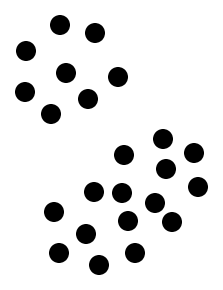
\includegraphics[width=0.5\linewidth]{graphics/cluster1.png}
    \caption{\label{fig:cluster_a}}
  \end{subfigure}
  \begin{subfigure}[b]{0.3\textwidth}
    \centering
    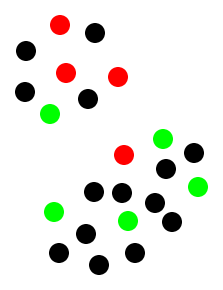
\includegraphics[width=0.5\linewidth]{graphics/cluster2.png}
    \caption{\label{fig:cluster_b}}
  \end{subfigure}
  \begin{subfigure}[b]{0.3\textwidth}
    \centering
    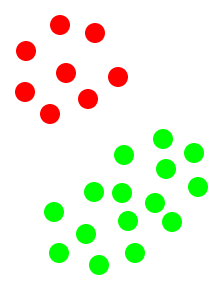
\includegraphics[width=0.5\linewidth]{graphics/cluster3.png}
    \caption{\label{fig:cluster_c}}
  \end{subfigure}
% 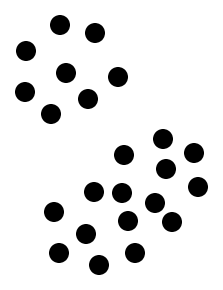
\includegraphics[width=0.3\textwidth]{graphics/cluster1.png}
% 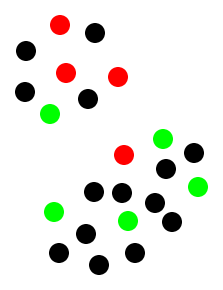
\includegraphics[width=0.3\textwidth]{graphics/cluster2.png}
% 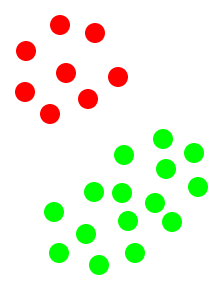
\includegraphics[width=0.3\textwidth]{graphics/cluster3.png}
\begin{tiny}
\caption{The process of exploiting cluster structure in data within active learning algorithm. In \ref{fig:cluster_a} we are supplied with some unlabeled data with obvious structure --- 2 clusters. In \ref{fig:cluster_b} we query for labels of some points from each cluster --- clusters are not pure, collected sample is noisy. In \ref{fig:cluster_c} we assign majority class to each cluster and arrive at presented model.\label{fig:cluster}}
\end{tiny}
\vspace{1cm}
\end{figure}


\begin{figure}[htbp]
\centering
  \begin{subfigure}[b]{0.3\textwidth}
    \centering
    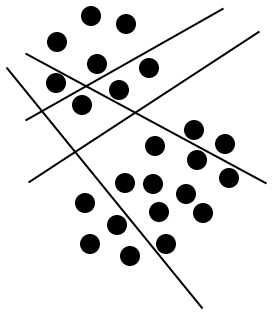
\includegraphics[width=0.5\linewidth]{graphics/hypsearch1.png}
    \caption{\label{fig:hypsearch_a}}
  \end{subfigure}
  \begin{subfigure}[b]{0.3\textwidth}
    \centering
    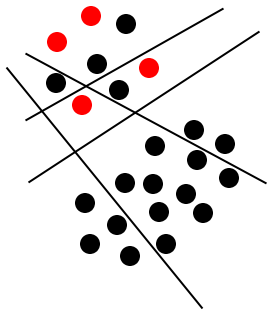
\includegraphics[width=0.5\linewidth]{graphics/hypsearch2.png}
    \caption{\label{fig:hypsearch_b}}
  \end{subfigure}
  \begin{subfigure}[b]{0.3\textwidth}
    \centering
    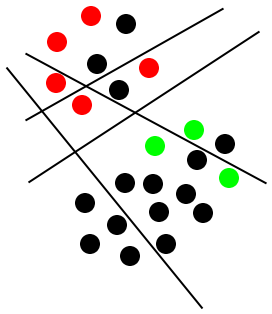
\includegraphics[width=0.5\linewidth]{graphics/hypsearch3.png}
    \caption{\label{fig:hypsearch_c}}
  \end{subfigure}
  \begin{subfigure}[b]{0.3\textwidth}
    \centering
    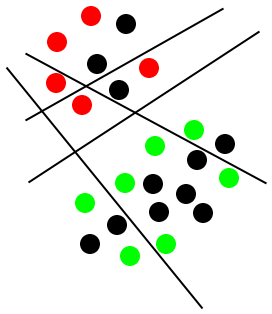
\includegraphics[width=0.5\linewidth]{graphics/hypsearch4.png}
    \caption{\label{fig:hypsearch_d}}
  \end{subfigure}
  \begin{subfigure}[b]{0.3\textwidth}
    \centering
    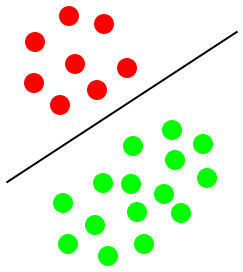
\includegraphics[width=0.5\linewidth]{graphics/hypsearch5.png}
    \caption{\label{fig:hypsearch_e}}
  \end{subfigure}
% 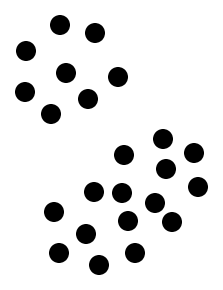
\includegraphics[width=0.3\textwidth]{graphics/cluster1.png}
% 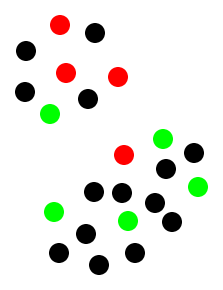
\includegraphics[width=0.3\textwidth]{graphics/cluster2.png}
% 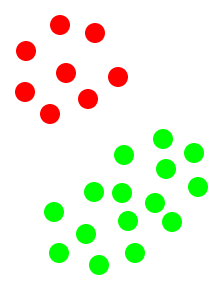
\includegraphics[width=0.3\textwidth]{graphics/cluster3.png}
\begin{tiny}
\caption{The process of search through hypothesis space within active learning algorithm. In \ref{fig:hypsearch_a} we select some hypothesis (~$h_i$~) that are potentially the best. To eliminate first we ask for a labels of points on both sides of $h_1$ and disregard it as on both sides we spot the same class (Figure \ref{fig:hypsearch_b}). In \ref{fig:hypsearch_c} and \ref{fig:hypsearch_d} we do the same for $h_2$ and $h_3$. We reject both of them with similar to previous observation. Finally, we arrive at hypothesis $h_5$ which agrees on all queried points and become output of our learning algorithm --- we assign to the rest of points majority class on given side of $h_5$.\label{fig:hypsearch}}
\end{tiny}
\vspace{1cm}
\end{figure}



\section{Active Learning in a view of Multi-Armed Bandits}
To build a ``bridge'' between MAB and AL we first need to describe settings of such scenario. For the sake of simplicity we focus on pool based, binary active learning with an approach of search through \emph{hypothesis space} $\mathscr{H}$, restricted by a query budget $B$. Moreover, we restrict our hypothesis space to linear classifiers(see later Section~\ref{sec:linearclassifiers}). The key point is to view learning problem as exploration-exploitation trade-off. We will first focus on finding connections between characteristic features of MAB and discover correspondence in AL.\\

To begin with, we will frame learning problem as $B$ round game --- finite horizon with discount sequence $\mathbf{A} = ( \underbrace{ 1, 1, 1, ..., 1}_{B}, 0, 0, 0, ... )$ --- where in each round agent is faced with pulling one of given arms and suffer some loss $L_t$ on chosen action. For simplicity, in this scenario we change reward for a loss what leads to optimal strategy being the one that minimizes loss instead of maximizing reward over $B$ rounds.\\

It is worth noting that if $B \rightarrow \infty$ then this becomes supervised algorithm which is fed by data stream.\\

To be more precise, we define equivalence between arms of a bandit and hypothesis $\mathit{h} \in \mathscr{H}$. We also need to find a proxy of MAB loss signal in our active learning scenario, but lets first clarify goals of our strategy.\\
The main aim is to estimate optimal hypothesis i.e.\ the one with lowest risk (loss) with use of as little labeled points as possible. If we knew the best $\mathit{h}$, so the one with minimal cumulative loss then the optimal strategy would be to pull this arm in each round of our experiment. This leads to the goal of finding optimal strategy as quickly as possible. Now we are left with defining a strategy telling us which arm to pull in each round and dilemma how to transform feedback --- in our case ground truth (genuine label) --- of queried point $x$ from our pull into a loss signal.\\

\subsection{Linear classifier\label{sec:linearclassifiers}}
To begin with, we define linear classifier as:
$$
c(x) = \mathbf{w} \cdot \mathbf{x} - t \text{~,~}
$$
where for binary classification we have:
$$
c(x) \geq 0 \rightarrow \text{ $x$ is assigned to $+$}
$$
$$
c(x) < 0 \rightarrow \text{ $x$ is assigned to $-$.}
$$\\

Where $\mathbf{w}$ is weight vector and $\mathbf{x}$ is data point with $\mathbf{x} \in \mathbb{R}^n$.\\
In general, linear model (hypothesis class) is concerned with finding the weight vector $\mathbf{w}$ such that our classifier is of the form given above. We can transform above equation to express decision boundary $t = \mathbf{w} \cdot \mathbf{x}$. This result tells us that decision boundary is a plane in the space spanned by $x_i \in \mathbf{x}$ variables. Where vector $\mathbf{w}$ is perpendicular to boundary and points in direction of $+$ class.\\
The notation of classifier can be simplified by extending both vectors $\mathbf{x}$ and $\mathbf{w}$ with $x_0 = 1$ and $w_0 = -t$ leading to decision boundary $c(x) = \mathbf{w}^{\circ} \cdot \mathbf{x}^{\circ} = 0$. In this form for the expense of one extra dimension we get decision boundary passing through origin of our coordinate system.\\
For visual example please see figure~\ref{fig:binclas}.\\

\begin{figure}[htbp]
  \centering
  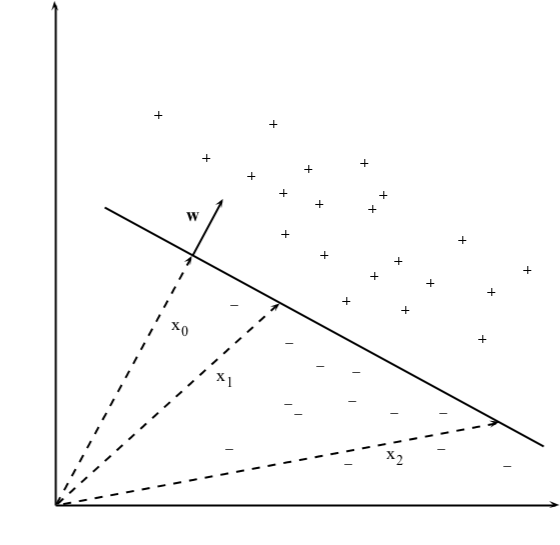
\includegraphics[width=0.5\linewidth]{graphics/binclas.png}
  \begin{tiny}
    \caption{Visualization of binary, linear classifier in two dimensions.\label{fig:binclas}}
  \end{tiny}
  \vspace{1cm}
\end{figure}

\subsection{Choosing best hypothesis}
To address the first mentioned above issue we refer to~\cite{DBLP:journals/corr/GantiG13} where an unbiased estimator of the risk of hypothesis is defined as:\\
$$
\hat{L}_t(a) = \frac{1}{Nt} \sum_{n=1}^{N} \sum_{\tau = 1}^{t} \frac{Q^{\tau}_n}{p^{\tau}_n} L(y_n h(\mathbf{x}_n)) \text{~,}
$$
where $p^t_n$ is probability of querying $\mathbf{x}_n$ in round $t$ extracted from vector $p^t$ described in section~\ref{sec:pointtoquery}.\\
Furthermore, $Q^t_n$ is a random variable which takes values $\{0,1\}$; $1$ if $\mathbf{x}_n$ was queried in round $t$ and $0$ otherwise.\\

We also need to decide on loss function to employ in our model. All loss functions which are convex w.r.t\ margin and which are upper bounded by $L_{\text{max}} < \infty$ will be suitable. For example we could use logistic loss, squared loss or exponential loss.\\

To sum up, each hypothesis in group of linear classifiers can be fully describe by weight vector $\mathbf{w}$. This observation allows us to notationally unify output of hypothesis $h_j$ on point $\mathbf{x}_n$ as $h_j(\mathbf{x}_n) = c(\mathbf{x}_n)$.\\


\subsection{Choosing a point to query --- Constructing loss signal\label{sec:pointtoquery}}
To iteratively improve our guess of best hypothesis we query possibly most informative point in each round. Intuitively such information allows us to tell apart good hypothesis which agree with acquired label and bad ones which mis-classify given point. To make the best possible choice we construct sampling distribution which minimizes the variance of the risk estimate $\hat{L}_t(h)$ defined above. We construct it by utilizing labels which we have already acquired from oracle and labels that our current hypothesis assigns to points which have not been queried yet. To guarantee infinite exploration of all hypothesis and avoid $0$ probabilities we introduce parameter $p_{min}$ which is arbitrarily set by user and denote minimum probability of each point being queried.\\

Let's define $\mathscr{Q}_t$ as a set of labels $y_n$ acquired by queering $\mathscr{O}$ for labels of $\mathbf{x}_n$ up to time $t$.\\
Just to recall we handle a binary classification which for data point $\mathbf{x}_n$ outputs result $c(\mathbf{x}_n)$. This result can be any real number, which is translated into class by rule given above: $c(\mathbf{x}_n) > 0 \rightarrow +$ and $c(\mathbf{x}_n) < 0 \rightarrow -$. As a notation shorthand it is often use $\textit{sign}(c(\mathbf{x}_n)) = y_n \in \{+, -\}$.\\

For each data point $\mathbf{x}_n \in \mathscr{P}$ in our pool we have:
$$
\hat{y}_n = \begin{cases}
                                    y_n = c(\mathbf{x}_n)  & \text{if } \mathbf{x}_n \in \mathscr{Q}_{t-1} \\
                                    \textit{sign}(h_t(\mathbf{x}_n)) & \text{otherwise.}
                                  \end{cases} 
$$

To decide which point to query we utilize introduced earlier loss and margin function; therefore setting $z(\mathbf{x}_n) = \hat{y}_n h_t(\mathbf{x}_n)$. Let's also note that cardinality of pool is: $|\mathscr{P}| = N$.\\
This leads to probability vector underlying sampling distribution being defined as:
$$
p_n^t = p_{\text{min}} + (1-Np_{\text{min}}) \frac{L(z(\mathbf{x}_n))}{\sum_{\mathbf{x}_n \in \mathscr{P}} L(z(\mathbf{x}_n))}
$$

Calculating $\hat{c}_t = h_t$ and $\\hat{y}$ for each $\mathbf{x}_n$ during arbitrary round $t$ allows us to utilize this information to calculate corresponding loss. The next stage is to create a vector $\mathbf{p}_t$ containing at n\ts{th} position $L(z(\mathbf{x}_n))$. Finally, we use it to construct sampling distribution to choose a point to query. Such approach has an advantage of being more prone to query points with small margin (large loss) w.r.t\ current hypothesis $h_t$ or points which have already been queried for label but on which $h_t$ suffers a large loss (simply does not agree).\\

After sampling $\mathbf{x}_n$ we check whether it was already queried in the past; if so we reuse already gained label. On contrary, if $\mathbf{x}_n$ has not been queried yet, we do so and increase our budget counter.


\subsection{Uncertainty of hypothesis}
The variance --- measure of uncertainty --- for risk (loss) of our hypothesis is calculated with help of calculated above vector for sampling distribution over pool instances as:
$$
U(\hat{L}_t(a)) = \frac{4}{Nt} \sqrt{\log\frac{1}{\delta}V_t}
$$
and
$$
V_t = \left[
\sum_{n = 1:N \\ \tau = 1:t} \frac{Q^\tau_n}{(p^\tau_n)^2} L^2(z(\mathbf{x}_n))
-
\left( \sum_{\mathscr{Q}_t} L(z(\mathbf{x}_n)) \right)^2
+
\frac{L^2_{\text{max}}  \sqrt{2t \log(\frac{1}{\delta}) (N-1)} } {\sqrt{p_{\text{min}}}}
\right]_+ \text{~,~}
$$

where $\delta$ is a parameter which is bounded by $\delta < \frac{1}{e}$.\\

This quantity together with previously defined estimator of the hypothesis risk was first defined in~\cite{DBLP:journals/corr/GantiG13}.\\


\subsection{Miscellaneous}
\subsubsection{Dealing with infinite hypothesis space}
Modeling huge or even infinite hypothesis space would suffer from existence of many arms in our bandit model leading to serious efficiency issue. Furthermore optimizing infinite space is not an easy task therefore we choose a subset of hypothesis space defined as:
$$
\mathscr{H} = \{ h : \|h\| \leq R \} \text{~,~}
$$
where $R$ is fixed such that $R > 0$ and $\| \dot \|$ is Euclidean $L_2$ norm.\\
Furthermore, based on observation described in~\cite{Abernethy08competingin} we have self-concordant barrier $\mathscr{R}(h)$ on $\mathscr{H}$ defined as:
$$
\mathscr{R}(h) = - \log(R^2 - \|h\|^2) \text{~.~}
$$
Given above restrictions allow us to significantly reduce dimensionality of hypothesis space by choosing hypothesis which differ. Moreover, presented barrier function is a continuous function which penalize with value close to $\infty$ hypothesis approaching defined boundary of hypothesis space.\\


\section{MAB-AL Algorithm}

In this section we will briefly discuss \texttt{MAB-AL} algorithm proposed in~\cite{DBLP:journals/corr/GantiG13} to familiarize reader with general concept which build upon presented in previous sections blocks.\\

\begin{algorithm}[H]
 \LinesNumbered
 \KwData{pool of points $\mathscr{P}$; loss function $L(\cdot)$; budget $B$; parameter $p_{min}$; access to oracle $\mathscr{O}$}
 \KwResult{optimal hypothesis $h_B$}
 $oracleQuerries = 0$\;
 $h_1 = 0$\;
 $t = 1$\;
 \While{oracleQuerries $\leq B$}{
  \For{$\mathbf{x}_n \in \mathscr{P}$}{
    $
    \hat{y}_n = \begin{cases}
      y_n = c(\mathbf{x}_n)  & \text{if } \mathbf{x}_n \in \mathscr{Q}_{t-1} \\
      \textit{sign}(h_t(\mathbf{x}_n)) & \text{otherwise.}
    \end{cases} 
    $ \;
    $p_n^t = p_{\text{min}} + (1-Np_{\text{min}}) \frac{L(z(\mathbf{x}_n))}{\sum_{\mathbf{x}_n \in \mathscr{P}} L(z(\mathbf{x}_n))}$ \;
  }
  sample point $\mathbf{x}$ from probability vector $\mathbf{p}^t$\;
  \eIf{$\mathbf{x}$ was already queried}{
   reuse label of $\mathbf{x}$\;
   }{
   query oracle $\mathscr{O}$ for the label $y = c(\mathbf{x})$ of $\mathbf{x}$\;
   $oracleQuerries \leftarrow oracleQuerries + 1$\;
  }
  solve: $h_{t+1} \leftarrow \text{argmin}_{h \in \mathscr{H}} LCB_t(h) + \lambda_t \mathscr{R}(h)$\;
  $t \leftarrow t + 1$\;
 }
 \caption{LCB-AL presented in~\cite{DBLP:journals/corr/GantiG13}.\label{LCB-AL}}
\end{algorithm}

% give the algorith and describe how it works


\section{Employing Thompson's Sampling}

% Do it


\section{Tweaks, Alternatives and Improvements --- Experiment}


\label{sec:qimprove}
How I would improve choice of point to query?\\
One way would be to change formula for margin to $z(x_i) = \hat{c}(x_i)  h_t(x_i) p_{\text{right}}(x_i, c_k)$.\\
Where $p_{\text{right}}(x_i, c_k)$ is the probability of hypothesis being correct with prediction.\\
BUT HOW TO CALCULATE IT???
We might use distribution of our hypothesis and take $p_{\text{right}}(x_i, c_k)$ as \emph{probability density function}!
END OF DISCOVERY FOR TODAY!\\

For the purpose of the experiment which may or may not be done by that time we can assume: see build bridge paper
$$
U(\hat{L}^\prime_t(a)) = \frac{ \sqrt{ \log(t) } }
                       { 10 }
                  \sqrt{ V^\prime_t }
$$
and
$$
V^\prime_t = \left[
  \sum_{i = 1:n \\ \tau = 1:t} \frac{Q^\tau_i}{(p^\tau_i)^2} L^2(z(x_i))
  -
  \left( \sum_{\mathscr{Q}_t} L(z(x_i)) \right)^2
\right]_+
$$~\\


We can use these estimations of mean and variance to model our Thompson's Sampling approach what will follow in next section.\\

Then next section with experiment design and we'll'ya see. Should be the end \\

And before experiment polish first chapter with berry and Firsted.


feasible --- just a word not a section



\appendix
\chapter{Code snippets}

\label{snip:normaldist}PDF of normal distribution with mean $0$ and standard deviation $5$.
\begin{lstlisting}
x   <- seq(-30,30,length=10000)
y   <- dnorm(x,mean=0, sd=5)
plot(x,y, type="l", lwd=1)
\end{lstlisting}

\label{snip:thompsonsampling}Creating multiple normal distributions to visualize Thompson sampling.
\begin{lstlisting}
 x   <- seq(5,15,length=1000)
 y   <- dnorm(x,mean=10, sd=30)
plot(x,y, type="l", lwd=1)
sam <- sample(x, 10)
points(sam,dnorm(sam, 10, 1), col="green")

# for a few distributions
\end{lstlisting}


\newpage
\begin{center} \textbf{\huge \vspace*{15pt} FIN~\cite{berry+firstedt}} \end{center}

\bibliography{ref}{}
\bibliographystyle{plain}

\end{document}
